\clearpage
\subsection{The Cosine Rule}

\begin{theorybox}{Notes}

The vertices of a triangle are labelled with capital letters, and the sides opposite each vertex are labelled with the corresponding lower-case letter.

\begin{center}
    \begin{tikzpicture}[scale=0.65]
        \draw (0,0) node[below left]{$A$} -- node[below right]{$c$}(6,2)node[right]{$B$} -- node[above right]{$a$} (2,5) node[above]{$C$} -- node[left]{$b$}cycle;
    \end{tikzpicture}
\end{center}

The Cosine Rule states:
$$ a^2 = b^2 + c^2 - 2bc \cos A $$
Similarly,
$$ b^2 = a^2 + c^2 - 2ac \cos B $$
and
$$ c^2 = a^2 + b^2 - 2ab \cos C. $$

To find an unknown angle slightly easier, the cosine rule can be re-arranged to give:

$$ \cos A = \dfrac{b^2 + c^2 - a^2}{2bc}$$

\end{theorybox}

\begin{pfbox}{Proof}

The diagram below shows triangle $ABC$ with side lengths $AC=b$, $BC=a$, and $AB=c$. We draw an altitude from $C$ to side $AB$ at point $D$.

\begin{center}
    \begin{tikzpicture}
        \coordinate[label=left:$A$] (A) at (0,0);
        \coordinate[label=right:$B$] (B) at (6,0);
        \coordinate[label=above:$C$] (C) at (4,3);
        \coordinate[label=below:$D$] (D) at (4,0);
        \draw (A) -- (B) -- node[above right]{$a$} (C) -- node[above left]{$b$} cycle;
        \draw[dashed] (C) -- node[right]{$h$} (D);
        \draw (3.8,0) -- (3.8,0.2) -- (4,0.2);
        \node at (2.2,-0.3) {$x$};
        \node at (5,-0.3) {$c-x$};
    \end{tikzpicture}
\end{center}

From right-angled triangle $ADC$:
\[
\cos A = \frac{x}{b} \quad \Rightarrow \quad x = b \cos A
\]
and
\[
h^2 = b^2 - x^2.
\]

From right-angled triangle $BDC$:
\[
a^2 = h^2 + (c-x)^2.
\]

Substituting for $h^2$:
\begin{align*}
    a^2 &= \left(b^2 - x^2\right) + (c-x)^2 \\
        &= b^2 - x^2 + c^2 - 2cx + x^2 \\
        &= b^2 + c^2 - 2cx.
\end{align*}

Substituting $x = b \cos A$ gives the cosine rule.:
\[
a^2 = b^2 + c^2 - 2bc \cos A.
\]
\end{pfbox}

\newpage

%% Worked Examples

\begin{examplecz}{Finding an unknown side}

In $\triangle ABC$, $AB=8$\,cm, $AC=6$\,cm and $\angle BAC=60^\circ$ as shown.
\begin{center}
    \begin{tikzpicture}[scale=0.9]
        \coordinate[label=left:$A$] (A) at (0,0);
        \coordinate[label=right:$B$] (B) at (6,0);
        \coordinate[label=above:$C$] (C) at (2.5,3.5);
        \draw (A) -- node[below]{$8$\,cm} (B) -- (C) -- node[left]{$6$\,cm} (A) -- cycle;
        \tkzLabelAngle[pos=1](B,A,C){$60^\circ$};
    \end{tikzpicture}
\end{center}
Find the length of $BC$, correct to two decimal places.
\tcblower
\textbf{Solution:}
\vspace*{40mm}
\begin{comment}
\begin{align*}
    BC^2 &= 6^2 + 8^2 - 2(6)(8)\cos 60^\circ \\
    &= 36 + 64 - 96(0.5) \\
    &= 100 - 48 \\
    &= 52 \\
    \therefore BC &= \sqrt{52} \approx 7.21\,\text{cm}.
\end{align*}
\end{comment}
\end{examplecz}

\vspace{3mm}

\begin{examplecz}{Finding an unknown angle}

In $\triangle XYZ$, $XY=9$\,cm, $YZ=11$\,cm and $XZ=14$\,cm.
\begin{center}
    \begin{tikzpicture}[scale=0.9]
        \coordinate[label=left:$X$] (X) at (0,0);
        \coordinate[label=right:$Y$] (Y) at (6,0);
        \coordinate[label=above:$Z$] (Z) at (3,4);
        \draw (X) -- node[below]{$9$\,cm} (Y) -- node[right]{$11$\,cm} (Z) -- node[above left]{$14$\,cm} (X) -- cycle;
        \tkzLabelAngle[pos=1](Y,X,Z){$\theta$};
    \end{tikzpicture}
\end{center}
Find the value of $\theta$, correct to one decimal place.
\tcblower
\textbf{Solution:}
\vspace*{40mm}
\begin{comment}
\begin{align*}
    11^2 &= 9^2 + 14^2 - 2(9)(14)\cos \theta \\
    121 &= 81 + 196 - 252 \cos \theta \\
    121 &= 277 - 252 \cos \theta \\
    252 \cos \theta &= 277 - 121 \\
    252 \cos \theta &= 156 \\
    \cos \theta &= \dfrac{156}{252} \\
    &= \dfrac{13}{21} \\
    \therefore \theta &= \cos^{-1}\left(\dfrac{13}{21}\right) \\
    &\approx 51.1^\circ
\end{align*}
\end{comment}
\end{examplecz}

\vspace{5mm}

%% Self-paced Questions

\begin{examplecz}{}

In $\triangle DEF$, $DE=7.2$\,cm, $DF=5.5$\,cm and $\angle EDF=47^\circ$.
\begin{center}
    \begin{tikzpicture}
        \coordinate[label=left:$D$] (D) at (0,0);
        \coordinate[label=right:$E$] (E) at (6,0);
        \coordinate[label=above:$F$] (F) at (3,3);
        \draw (D) -- node[below]{$7.2$\,cm} (E) -- (F) -- node[above left]{$5.5$\,cm} (D) -- cycle;
        \tkzLabelAngle[pos=1](E,D,F){$47^\circ$};
    \end{tikzpicture}
\end{center}
Find the length of $EF$, correct to one decimal place.
\tcblower
\textbf{Solution:}
\vspace*{4.25cm}
\end{examplecz}

\vspace{3mm}

\begin{examplecz}{}

In $\triangle GHI$, $GH=12$\,cm, $HI=9$\,cm and $GI=10$\,cm.
\begin{center}
    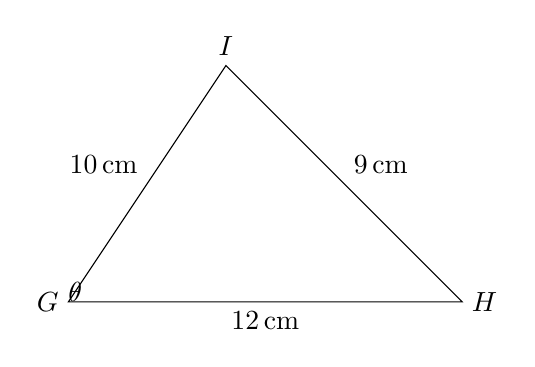
\begin{tikzpicture}
        \coordinate[label=left:$G$] (G) at (0,0);
        \coordinate[label=right:$H$] (H) at (5,0);
        \coordinate[label=above:$I$] (I) at (2,3);
        \draw (G) -- node[below]{$12$\,cm} (H) -- node[above right]{$9$\,cm} (I) -- node[above left]{$10$\,cm} (G) -- cycle;
        \tkzLabelAngle[pos=1](H,G,I){$\theta$};
    \end{tikzpicture}
\end{center}
Find the size of angle $\theta$, correct to the nearest degree.
\tcblower
\textbf{Solution:}
\vspace*{4.25cm}
\end{examplecz}

\newpage

\begin{examplecz}{}
Two jetskis depart from point $P$ at the same time. Jetski $A$ travels $3.6$\,km north and jetski $B$ travels $6$\,km on a bearing of $028^{\circ}$.
\vskip3mm
Using only the cosine rule, find the distance (to two decimal places), and bearing (to the nearest degree) of jetski $B$ from jetski $A$.
\tcblower
\textbf{Solution:}
\vspace{10cm}
\begin{comment}
\begin{center}
    \begin{tikzpicture}
        \coordinate[label=left: $P$] (P) at (0,0);
        \coordinate[label=above left: $A$] (A) at (0,3.6);
        \coordinate[label=above right: $B$] (B) at (2.82,5.3);
        \draw (P) -- node[left]{$3.6$\,km}(A) -- (B) -- node[below right]{$6$\,km} cycle;
        \tkzLabelAngle[pos=1.4](B,P,A){$28^{\circ}$};        
    \end{tikzpicture}
\end{center}
\end{comment}
\end{examplecz}

\vfill

\begin{Qbox}{}
    From \textit{CambridgeMaths Year 11 Mathematics Extension 1}:
    \begin{itemize}
        \item Exercise 6J: 1 to 7, 11
    \end{itemize}
\end{Qbox}